\section{Introdução}

A modução é um tecnica que permite a transmissão de sinais analógicos ou digitais através de um meio físico, como o ar ou cabos.
Segundo \cite{b12}, a modulação AM é um processo que envolve a variação da amplitude de uma portadora de alta frequência em função de um sinal modulante, que contém a informação a ser transmitida. Essa técnica é amplamente utilizada em sistemas de comunicação, como rádio e televisão, devido à sua simplicidade e eficácia na transmissão de sinais analógicos.


\subsection{Modulação AM-DSB-SC (Double Sideband Suppressed Carrier)}
A modulação AM-DSB (Double Sideband) é uma forma de modulação em que a portadora e as duas laterais (superior e inferior) são transmitidas. Esse tipo de modulação consiste em multiplicar o sinal de informação por uma portadora, como o sinal mensagem é de banda limitada, isto é, se o sinal $m(t)$ admite transformada de fourier, então $M(f) = 0$ para $|f| > W$, onde $W$ é a largura de banda do sinal.
Como a mensagem tem sua representação espectral, é possivel deslocar a mensagem para uma nova frequência utilizando a propriedade de modulação da transformada de Fourier, que nos diz que a multiplicação no domínio do tempo por uma exponencial complexa resulta em um deslocamento espectral no domínio da frequência. Multplicando o sinal de informação $m(t)$ por uma portadora $c(t) = A_{c} \cos(2 \pi f_{c} t)$, temos:
\begin{equation}
    s(t) = m(t) c(t) = A_{c} m(t) \cos(2 \pi f_{c} t)
\end{equation}

onde $A_{c}$ é a amplitude da portadora e $f_{c}$ é a frequência da portadora. Podemos expandir a expressão acima utilizando a identidade trigonométrica $\cos(x) = \frac{e^{jx} + e^{-jx}}{2}$, resultando em:

\begin{equation}
    s(t) = \frac{A_{c}}{2} m(t) e^{j 2 \pi f_{c} t} + \frac{A_{c}}{2} m(t) e^{-j 2 \pi f_{c} t}
\end{equation}

pode-se aplicar a transformada de Fourier em ambos os lados da equação, resultando em:

\begin{equation}
    S(f) = \frac{A_{c}}{2} (M(f - f_{c}) + M(f + f_{c}))
\end{equation}
Por exemplo, para uma mensagem $\cos(2\pi f_{m} t)$ com frequência $f_{m} = 100\,\text{Hz}$, uma portadora $\cos(2\pi f_{c} t)$ de $f_{c} = 1\,\text{kHz}$ com amplitude $A_{c} = 1$, realizando a modulação AM-DSB, os espectros para a mensagem, portadora e sinal modulado são mostrados nas Figuras~\ref{fig:espectro_mensagem}, \ref{fig:espectro_portadora} e \ref{fig:espectro_modulado}, respectivamente. O espectro do sinal modulado AM-DSB apresenta duas bandas laterais, uma superior e outra inferior, que contêm a mesma informação, além da portadora.

\begin{figure}[h]
    \centering
    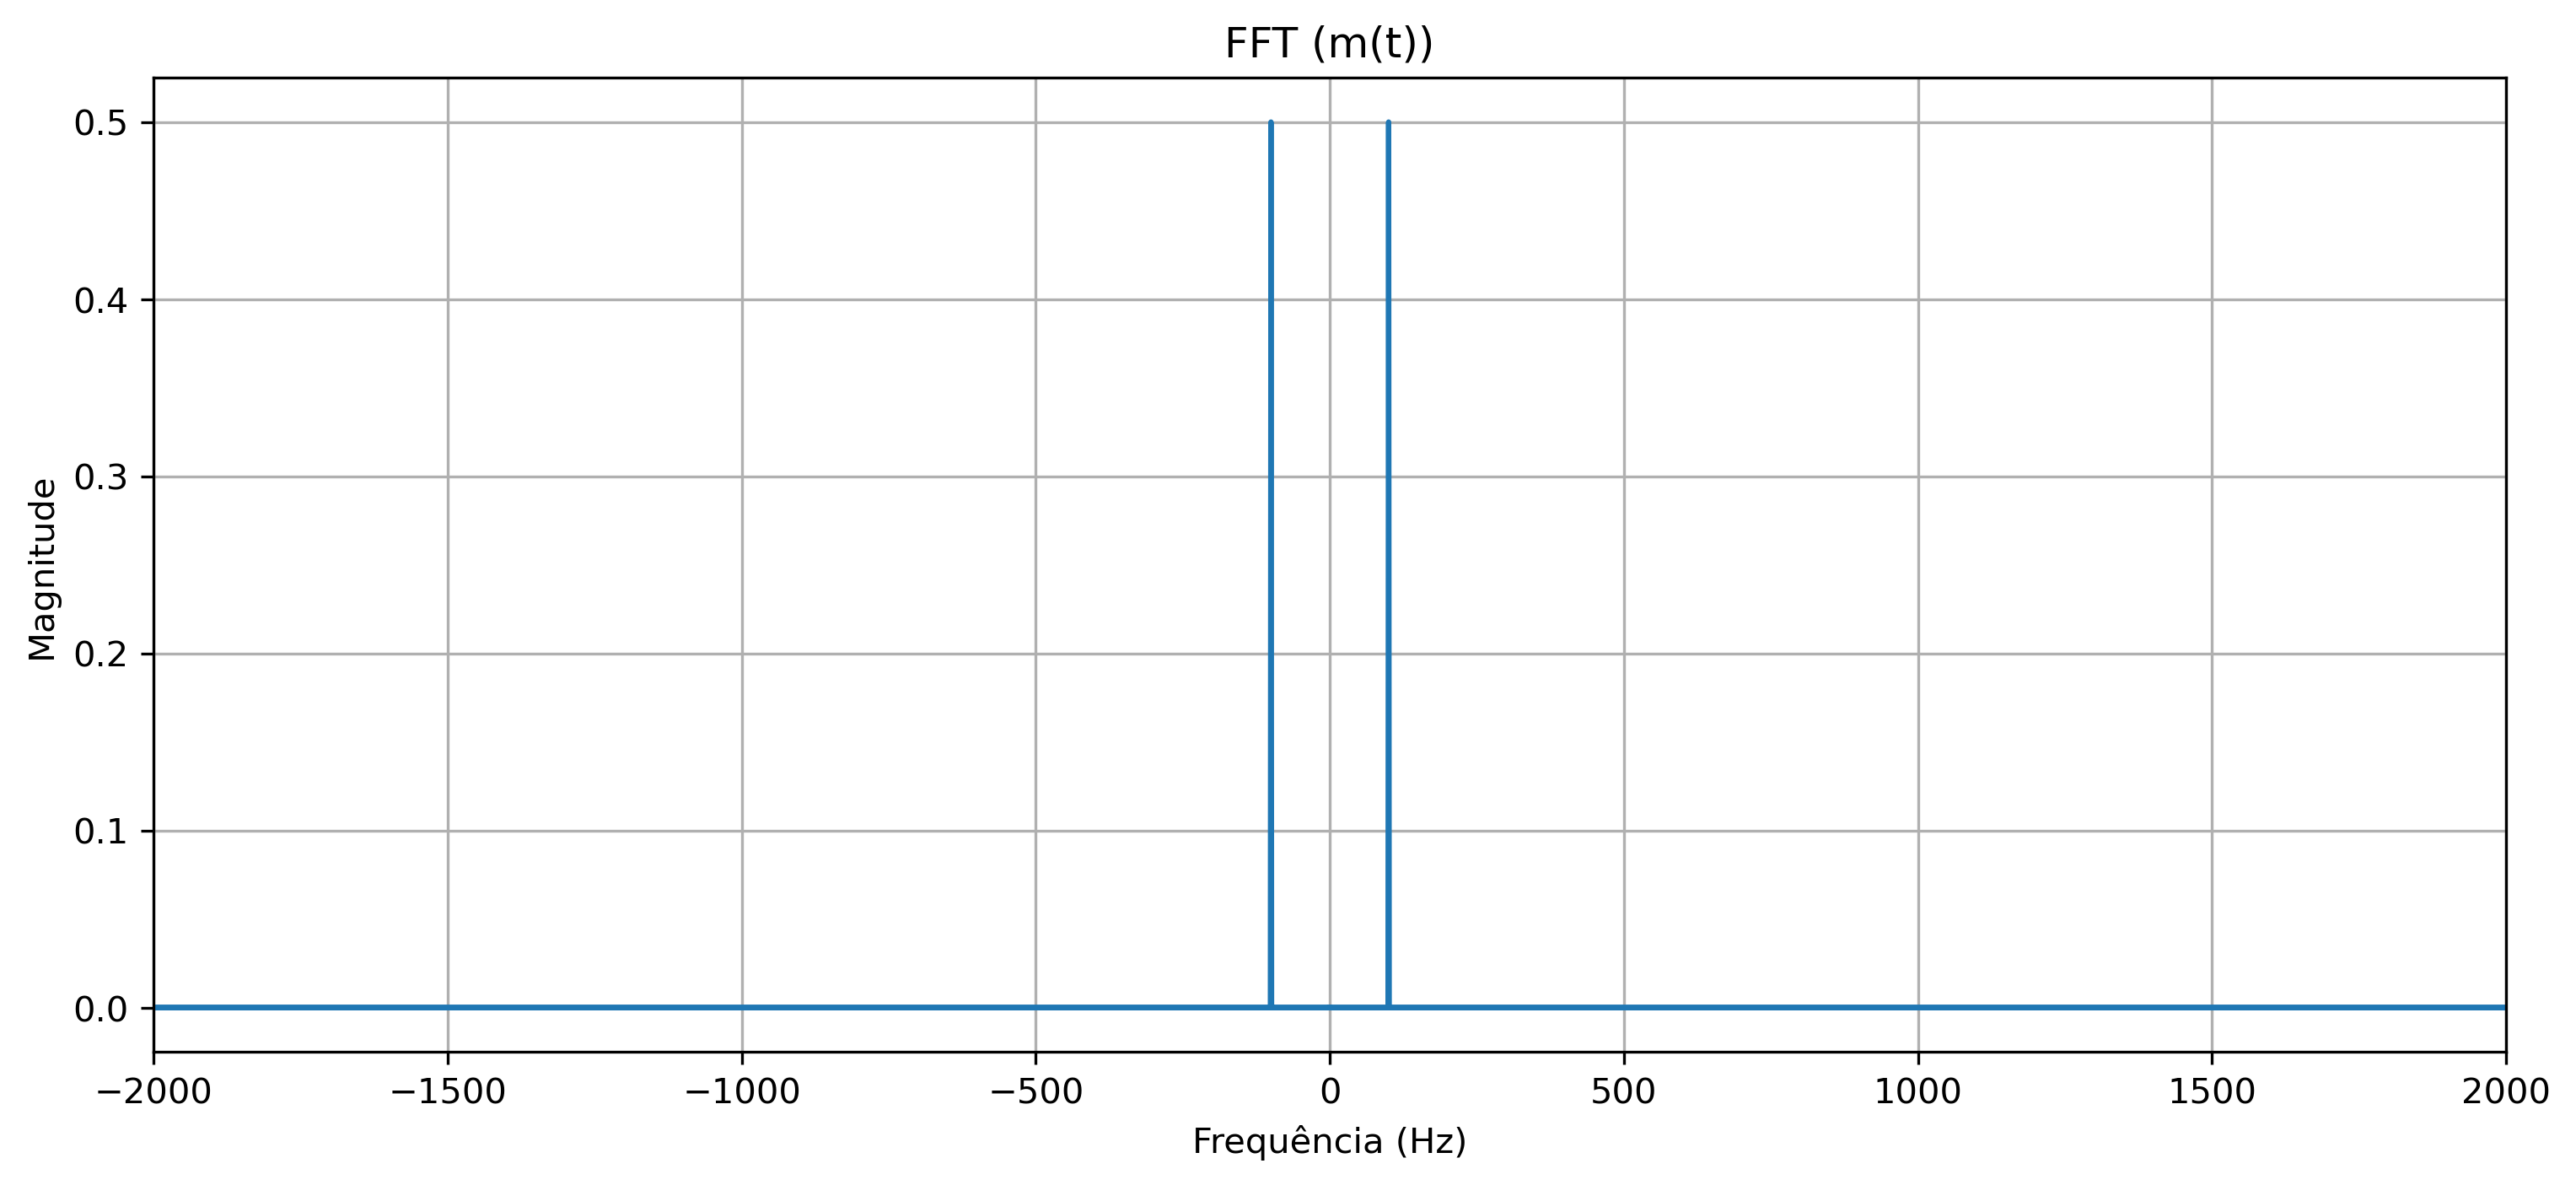
\includegraphics[width=0.5\textwidth]{images/FFT (m(t))_full.png}
    \caption{Espectro do sinal de mensagem. Fonte: Autor.}
    \label{fig:espectro_mensagem}
    \centering
\end{figure}

\begin{figure}[h]
    \centering
    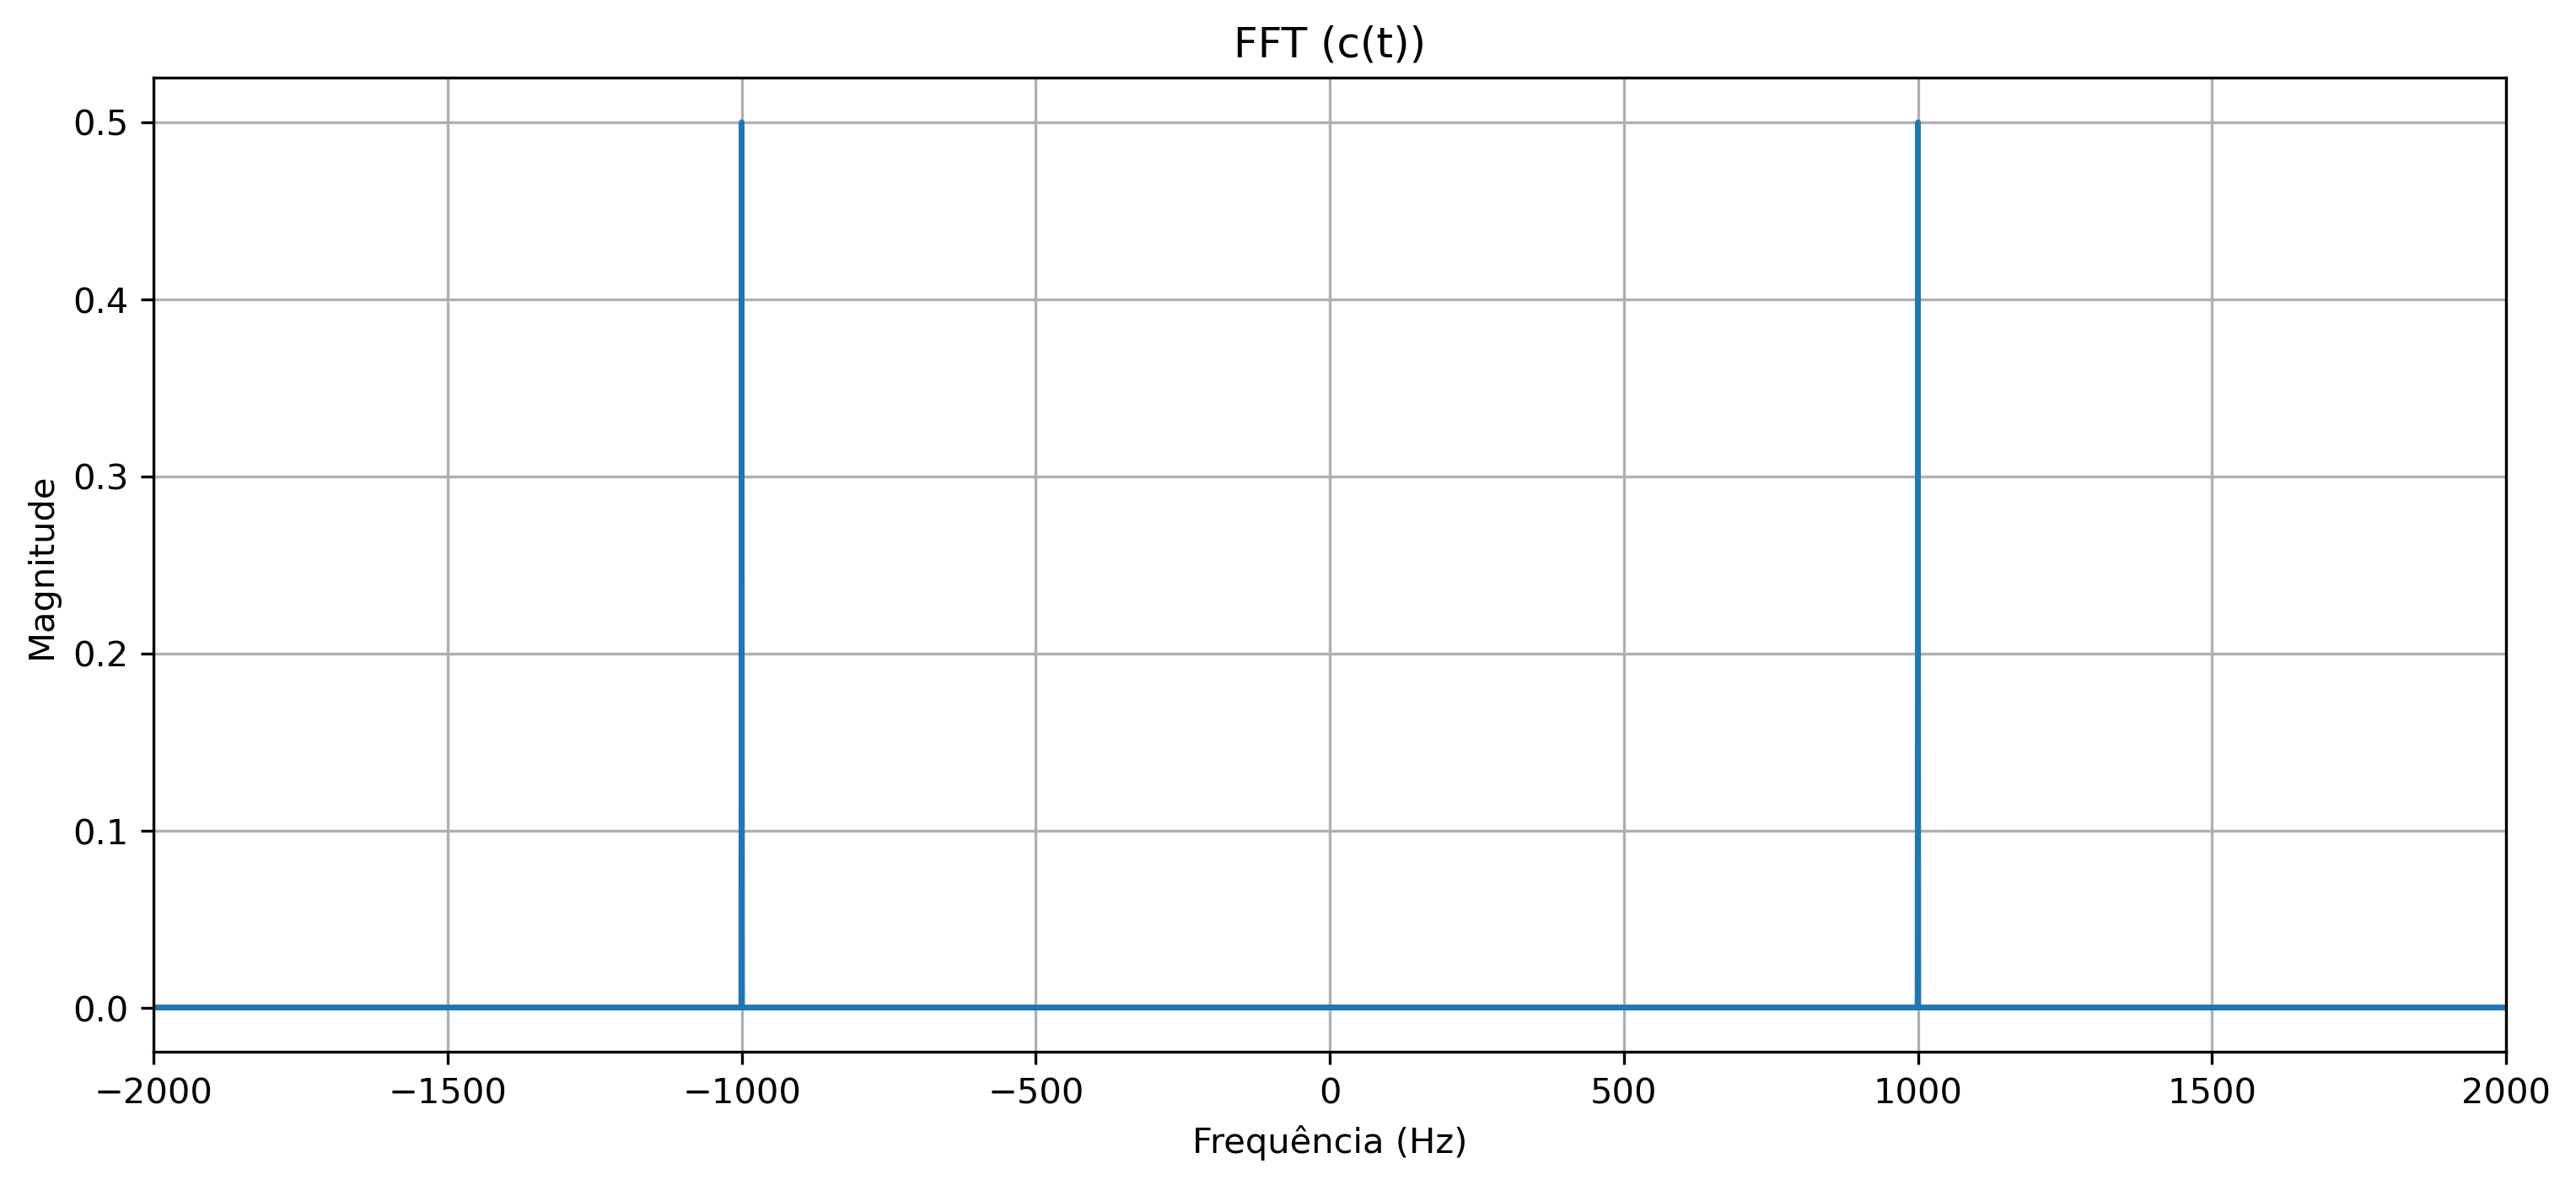
\includegraphics[width=0.5\textwidth]{images/FFT (c(t))_full.png}
    \caption{Espectro da portadora. Fonte: Autor.}
    \label{fig:espectro_portadora}
    \centering
\end{figure}

\begin{figure}[h]
    \centering
    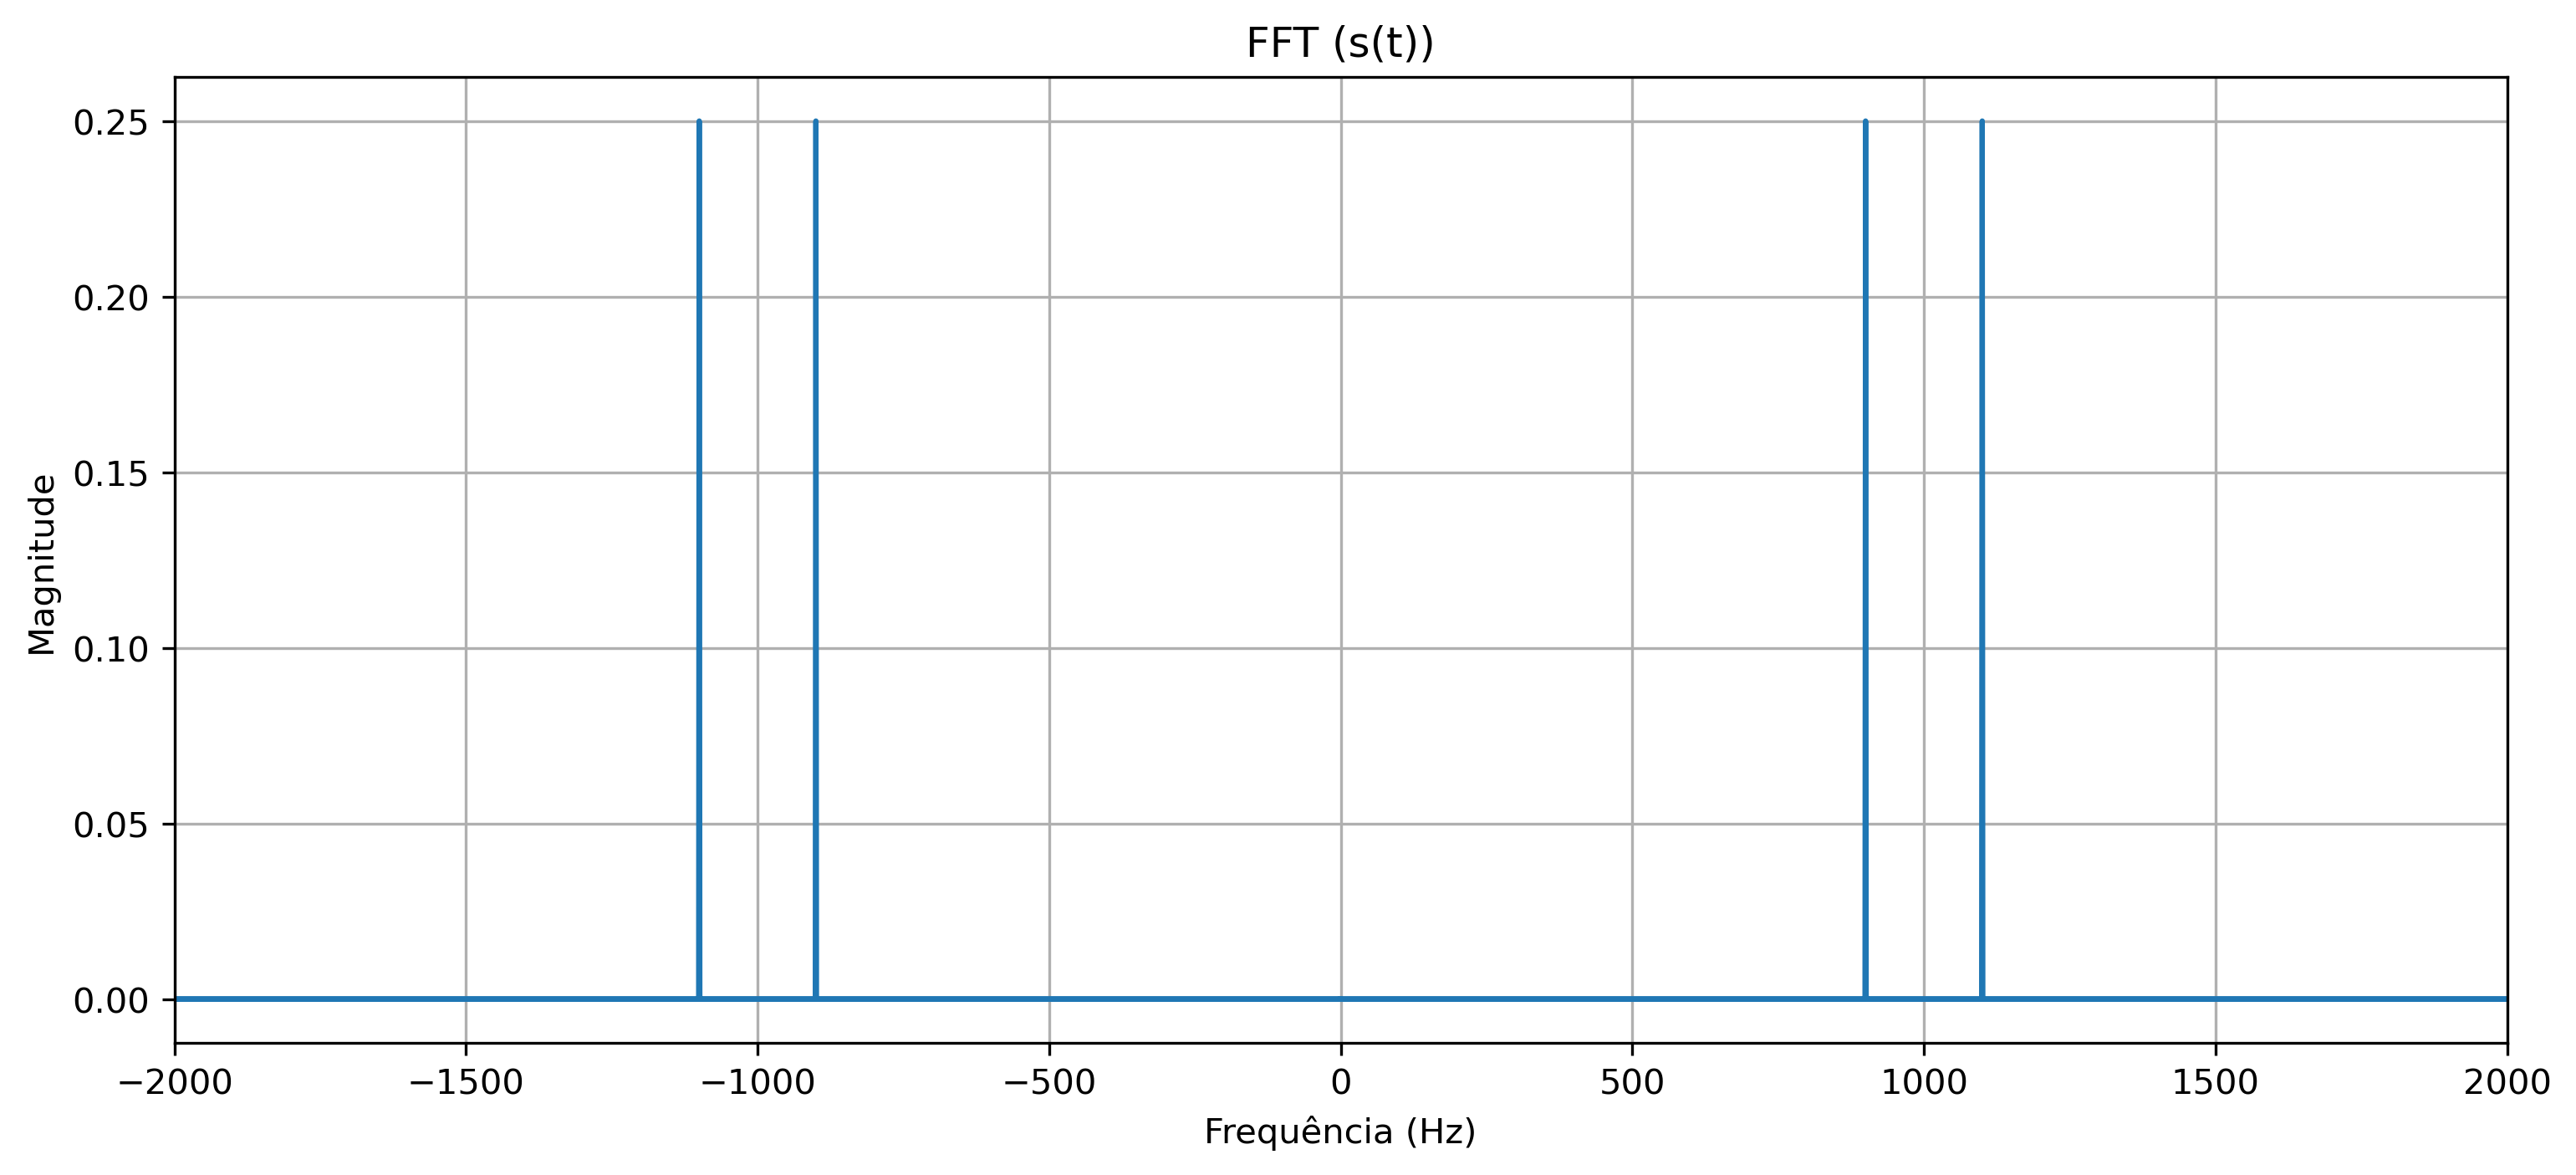
\includegraphics[width=0.5\textwidth]{images/FFT (s(t))_full.png}
    \caption{Espectro do sinal modulado AM-DSB. Fonte: Autor.}
    \label{fig:espectro_modulado}
    \centering
\end{figure}


O diagrama de blocos da modulação AM-DSB é apresentado na Figura \ref{fig:modulacao_am}, onde o sinal de informação $m(t)$ é multiplicado pela portadora $c(t)$, resultando no sinal modulado $s(t)$. A demodulação do sinal AM-DSB pode ser realizada utilizando um detector de envoltória, que recupera o sinal de informação original a partir do sinal modulado.

\begin{figure}[h]
    \centering
    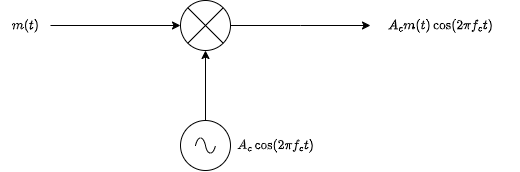
\includegraphics[width=0.5\textwidth]{images/modulacao_am.png}
    \caption{Diagrama de blocos da modulação AM-DSB. Fonte: Autor.}
    \label{fig:modulacao_am}
\end{figure}


Podemos demostrar os resultados a partir da transformada de Fourier, onde a transformada de Fourier do sinal modulado $m(t)$ é dada por:

\begin{equation}
    M(f) = \frac{1}{2} \left( \delta (f - 100) + \delta (f + 100) \right)
\end{equation}

substituindo na equação (3), temos:

\begin{align}
    S(f) = \frac{1}{4} \big(
        &\ \delta (f - 100 - 1000) + \delta (f + 100 - 1000) \notag \\
        &+ \delta (f - 100 + 1000) + \delta (f + 100 + 1000)
    \big)
\end{align}

Conforme mostrado no espectro \ref{fig:espectro_modulado}, a portadora é suprimida.


\subsection{demodulação AM-DSB-SC (Double Sideband Suppressed Carrier)}

A demodulação AM-DSB-SC é um processo que visa recuperar o sinal de informação original a partir do sinal modulado. O método mais comum para realizar essa demodulação é o uso de um multiplicador, que multiplica o sinal modulado por uma cópia da portadora. Esse processo resulta em um sinal que contém a informação original, mas também inclui uma componente de alta frequência que deve ser filtrada.

\begin{equation}
    s(t) = m(t) c(t) = A_{c} m(t) \cos(2 \pi f_{c} t)
\end{equation}

\begin{equation}
    y(t) = s(t) c(t) \cos(2 \pi f_{c}t)= A_{c} m(t) \cos(2 \pi f_{c} t)^{2}
\end{equation}

Linarizando o coseno, tempos:

\begin{equation}
    r(t) = \frac{A_{c}}{2} m(t) + \frac{A_{c}}{2} m(t) \cos(4 \pi f_{c} t)
\end{equation}

A transformada de Fourier do sinal demodulado $r(t)$ é dada por:

\begin{equation}
    Y(f) = \frac{A_{c}}{2} M(f) + \frac{A_{c}}{2} M(f - 2 f_{c}) + \frac{A_{c}}{2} M(f + 2 f_{c})
\end{equation}

Aplicando um filtro passa-baixa com largura de banda $W$ para eliminar a componente de alta frequência, obtemos o sinal de informação original:

\begin{equation}
    Y_{LPF}(f) = \frac{A_{c}}{2} M(f)
\end{equation}

O sinal é recuperado com uma amplitude reduzida, o que pode ser compensado por um amplificador. O diagrama de blocos da demodulação AM-DSB-SC é apresentado na Figura \ref{fig:demodulacao_am}, onde o sinal modulado $s(t)$ é multiplicado pela portadora $c(t)$, resultando no sinal demodulado $r(t)$. Em seguida, um filtro passa-baixa é aplicado para recuperar o sinal de informação original.

\begin{figure}[h]
    \centering
    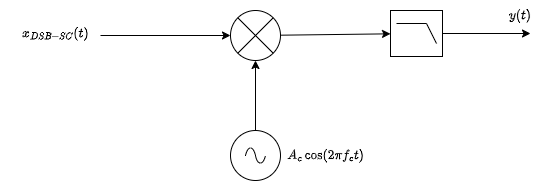
\includegraphics[width=0.5\textwidth]{images/demodulacao_am.png}
    \caption{Diagrama de blocos da demodulação AM-DSB-SC. Fonte: Autor.}
    \label{fig:demodulacao_am}
\end{figure}

Um dos principais desafios da modulação em amplitude com portadora suprimida (DSB-SC) é a necessidade de sincronização de fase entre o sinal modulado e a portadora na demodulação. Caso haja um desvio de fase entre a portadora original e a gerada no receptor, o sinal demodulado apresentará distorções significativas. Para mitigar esse problema, uma abordagem comum é transmitir um tom piloto juntamente com o sinal modulado. Esse tom é uma pequena fração da portadora original, inserida com baixa amplitude, e pode ser isolado no receptor por meio de um filtro de banda estreita. No entanto, a presença do tom piloto implica que a portadora não está totalmente suprimida, o que descaracteriza a modulação como DSB-SC pura.

Outra alternativa mais robusta é o uso de um PLL (Phase-Locked Loop), um circuito que sincroniza automaticamente a fase da portadora local com a fase do sinal modulado recebido. O PLL ajusta continuamente a frequência e a fase do oscilador local, permitindo uma demodulação mais precisa mesmo na presença de ruídos e desvios de fase. A Figura \ref{fig:demodulacao_am_pll} ilustra o esquema de demodulação utilizando PLL.

\begin{figure}[h]
    \centering
    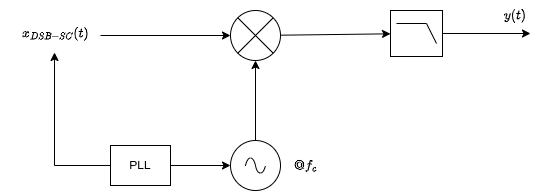
\includegraphics[width=0.5\textwidth]{images/demodulacao_am_pll.png}
    \caption{Diagrama de blocos da demodulação AM-DSB-SC com PLL. Fonte: Autor.}
    \label{fig:demodulacao_am_pll}
    \centering
\end{figure}




